\chapter{Desarrollo experimental}
\section{Construcción de la pecera y caracterización}
Se construyó un acuario rectangular utilizando vidrio laminado de 5+5 para la base y 3+3 para las paredes. Las dimensiones totales (internas) son (80x68x15)cm. La profundidad total de agua utilizada para las mediciones es $(12,4\pm0,1)$cm y no fue variada a lo largo del proyecto; el volumen de agua utilizado rondó siempre los 67l. El laminado de 5+5 soporta una columna de 80cm de agua por metro cuadrado, con lo cual la elección del material es por demás segura. El parlante se coloca en un extremo del acuario, en el medio y montado sobre una estructura de goma espuma. En la figura \ref{fig:acuario} se puede observar una fotografía de la pecera cargada con agua y el parlante colocado (sin neoprene). Este desarrollo fué el primer paso realizado en Laboratorio 6.

\begin{figure}[H]
	\centering
		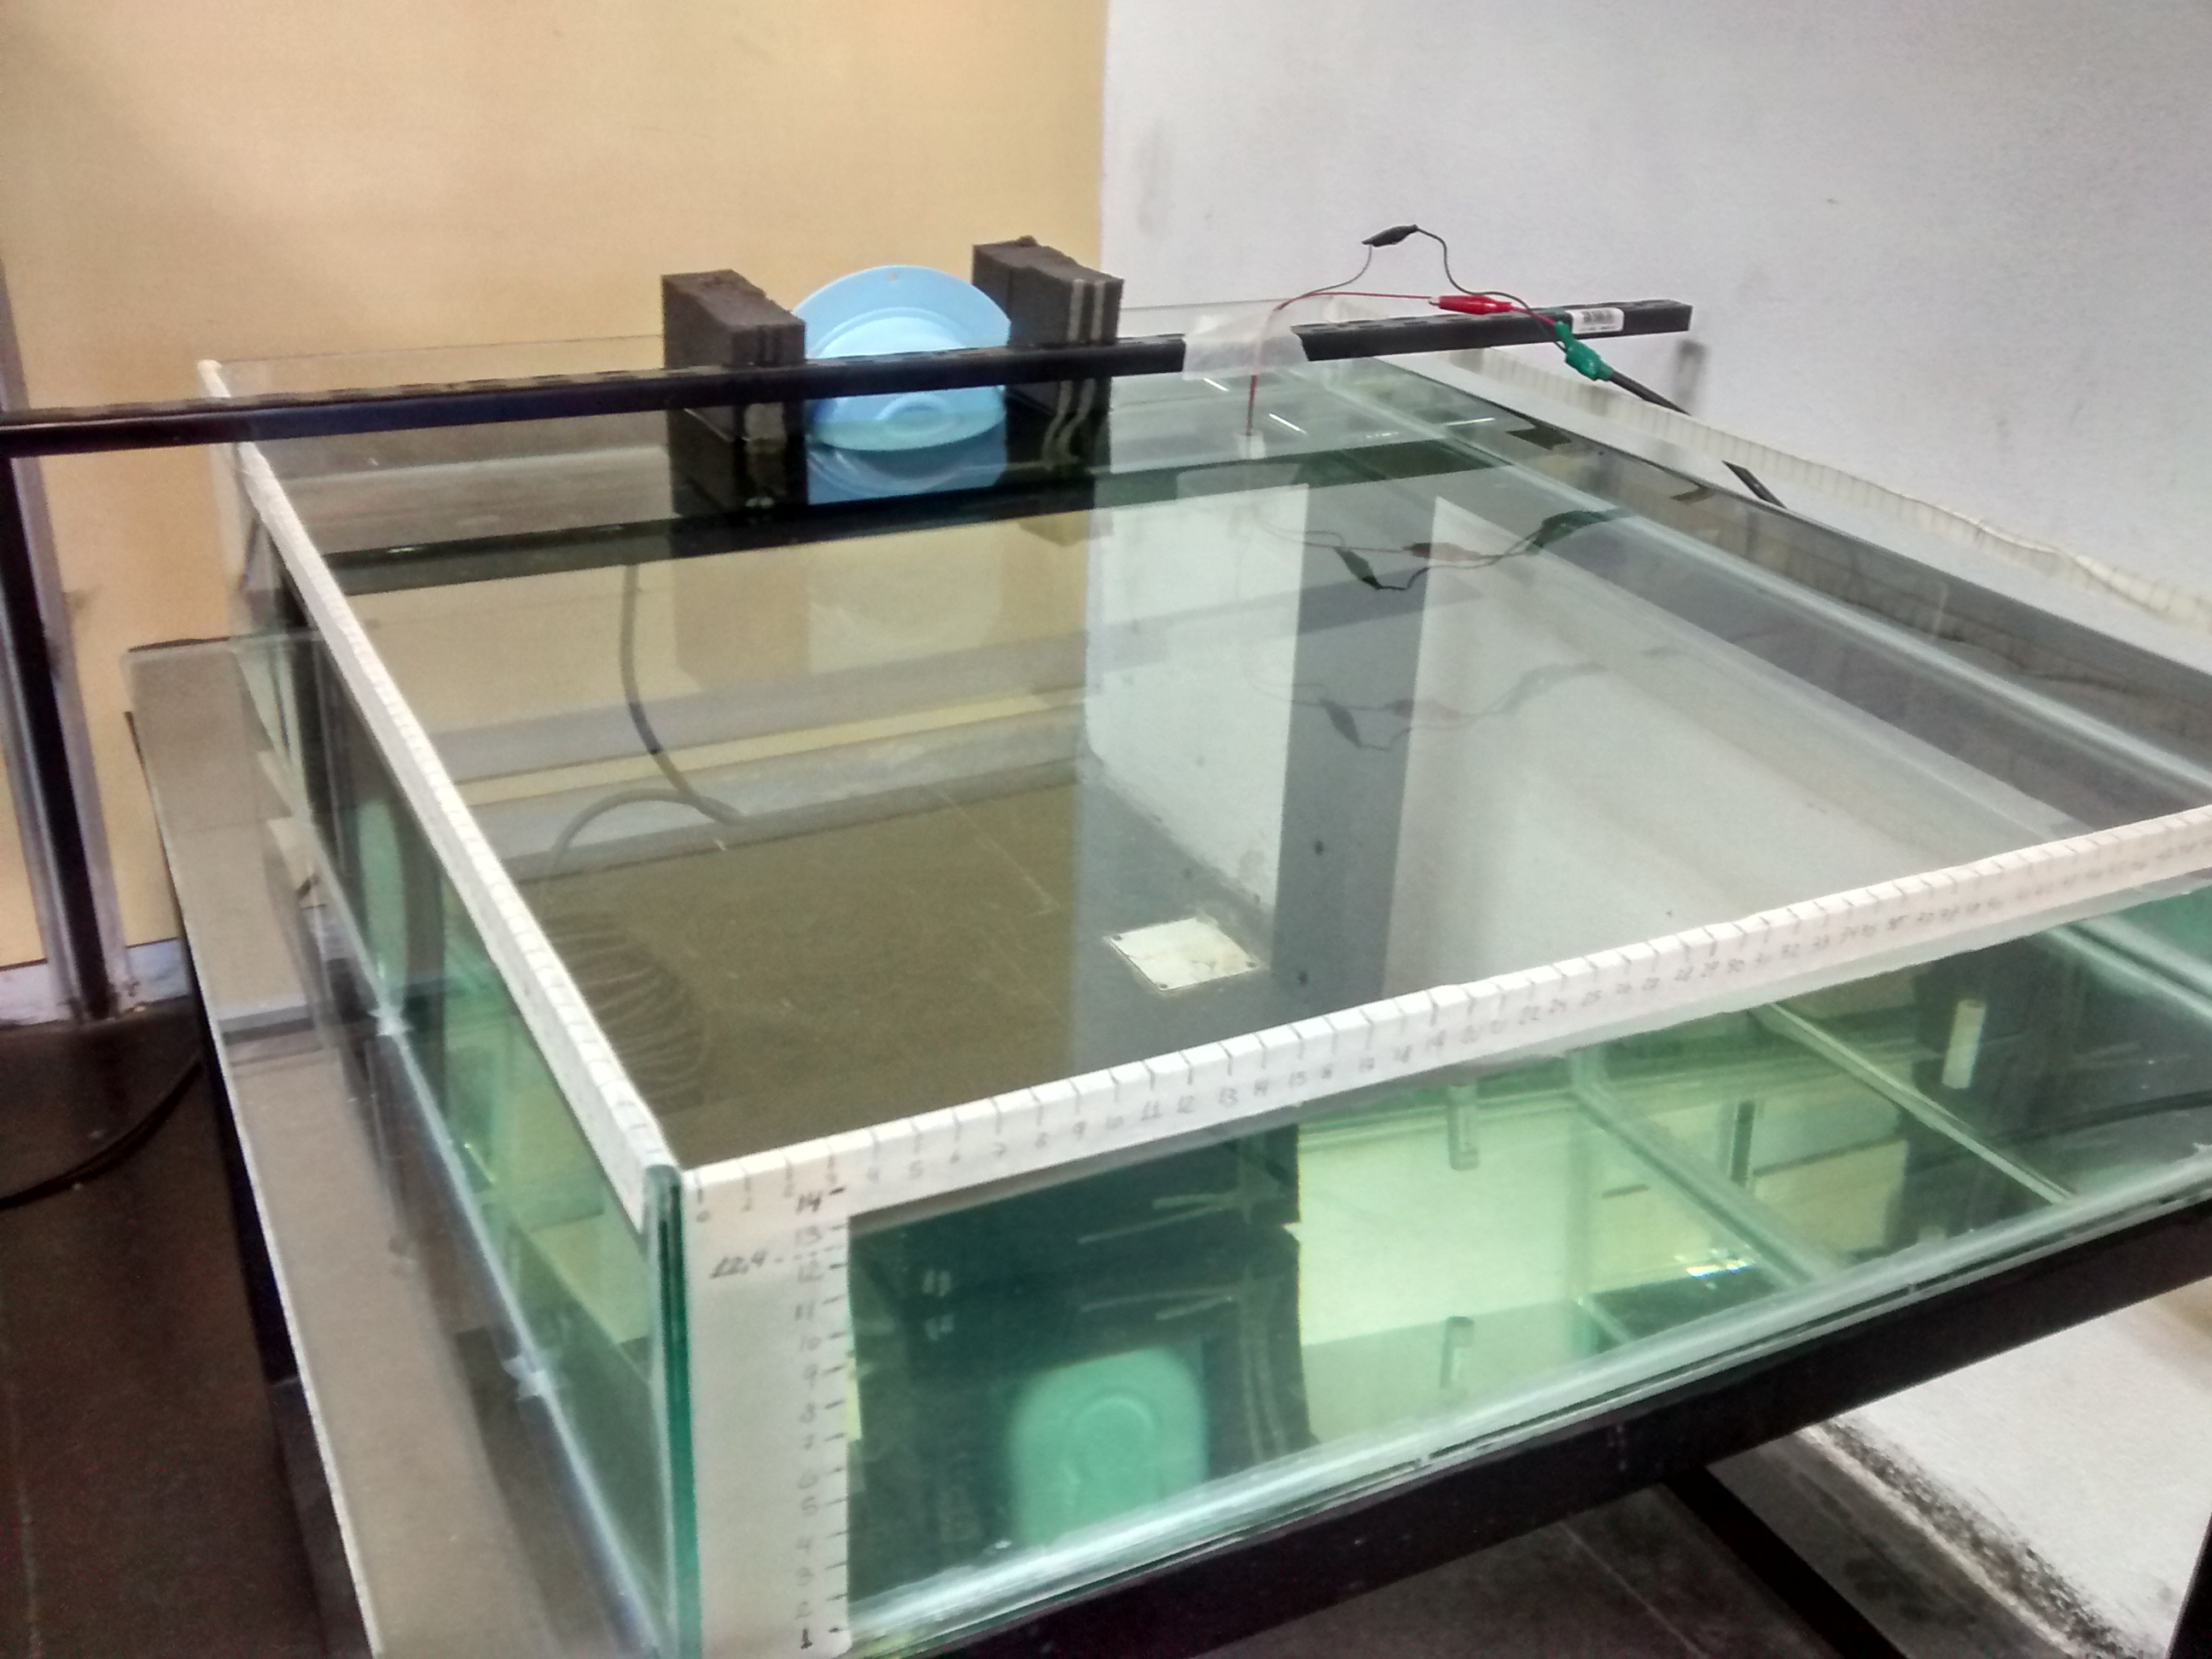
\includegraphics[height=6cm]{pecera.jpg}
		\caption{Fotografía del acuario donde se pueden observar el parlante (celeste) y un hidrófono (montado sobre la barra negra).}
	\label{fig:acuario}
\end{figure}

Para la caracterización se tomó una grilla de puntos en el acuario sobre los cuales se midió la RI mediante el proceso de deconvolución de barridos detallado en la sección \ref{sec:introsweeps}. En la figura \ref{fig:grilla} se muestra un esquema del acuario donde se observan, marcadas en rojo, las posiciones donde se ha caracterizado la RI. La grilla comienza a $(30\pm1)$cm del frente del parlante y avanza cada $(4\pm1)$cm hasta $(62\pm1)$cm respecto del parlante. En la otra dirección, se realizaron 16 mediciones equiespaciadas en $(3,0\pm0,5)$cm, empezando a $(10,0\pm0,5)$cm de una de las paredes.

\begin{figure}[H]
	\centering
		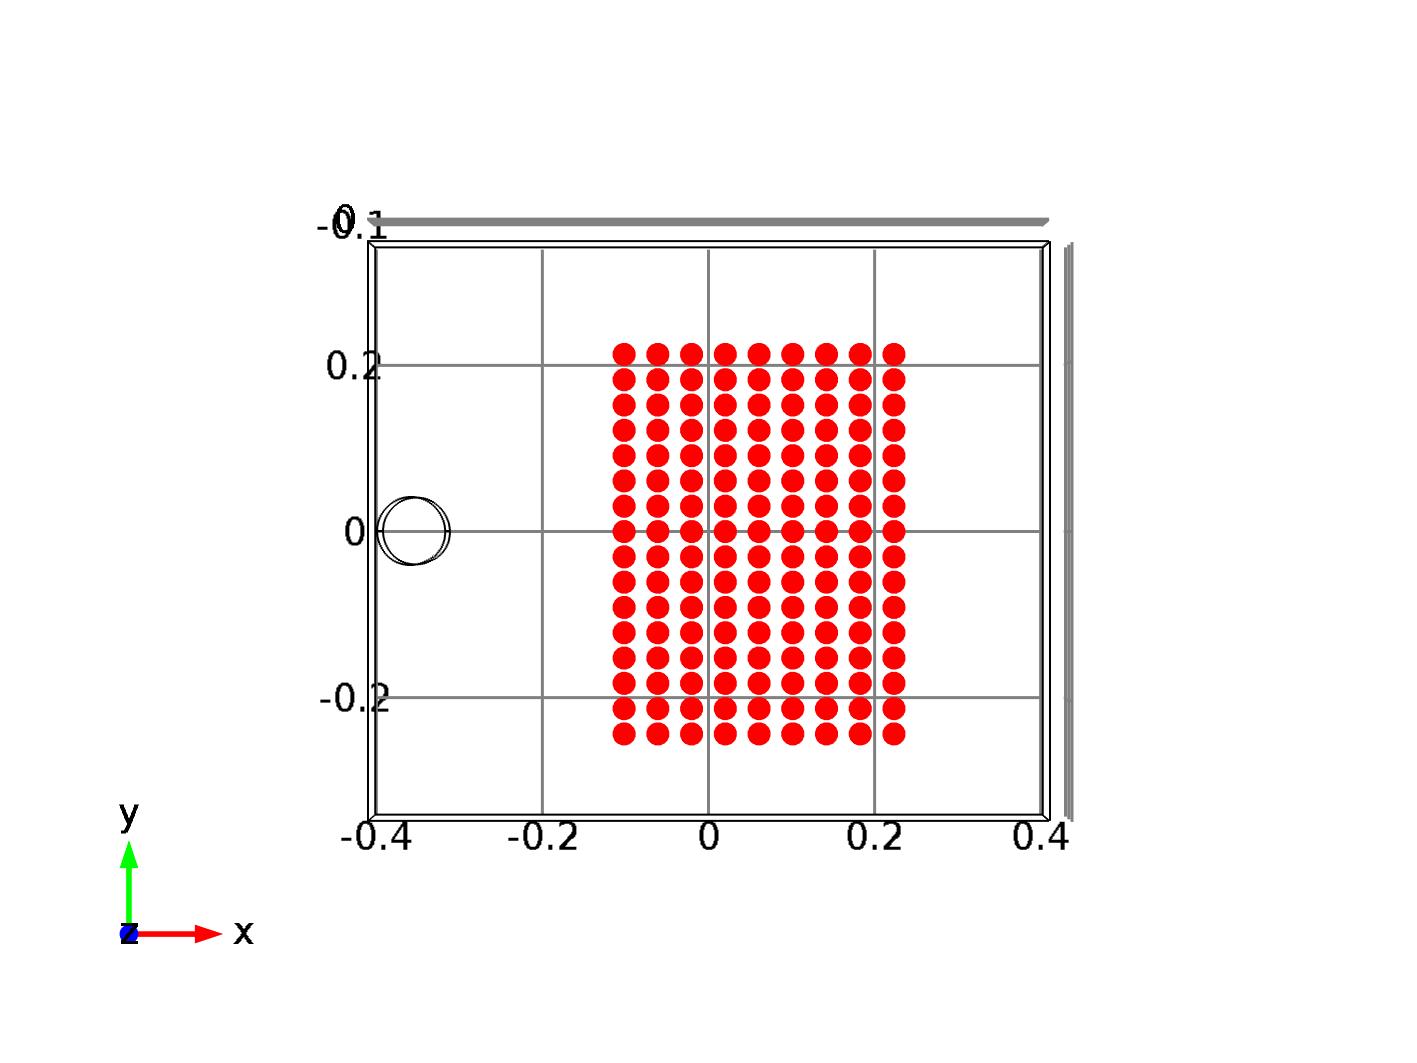
\includegraphics[height=7cm]{puntosmedidos.png}
		\caption{Grilla de puntos donde se caracterizó la RI.}
	\label{fig:grilla}
\end{figure}

El proceso de caracterización consiste entonces en:
\begin{enumerate}
	\item Generar un barrido y su filtro inverso con un script en Matlab. Los scripts fueron desarrollados por Oygo Sound LLC con las ecuaciones de [MullerMassarani] y puede bajarse de [6]. El barrido utilizado dura 20s y comprende un rango de frecuencias desde 400Hz hasta 10kHz. La frecuencia de muestreo es de 48kHz y se mantuvo esa misma frecuencia de muestreo para todas las grabaciones del proyecto (tanto las realizadas en Laboratorio 6 como Laboratorio 7).
	\item El hidrófono (SQ34, Sensor Technology) se conecta a la PC mediante un amplificador diferencial de ganancia 20x.
	\item El parlante se conecta a la PC mediante un amplificador de audio de 8$\Omega$ de impedancia y 30W máximo de salida. La amplificación utilizada para la caracterización fué de alrededor de $\approx$ 22W.
	\item Con el hidrófono en cada una de las posiciones de la grilla, se reproduce y graba en simultáneo el barrido y su respuesta utilizando el programa Audacity. La elección del programa radica en su facilidad de uso y la eficiencia de recursos de la PC para grabar durante todo el día.
	\item Finalmente, se procesa la grabación con el filtro inverso para obtener la respuesta impulso. Un script en Python realiza la convolución mediante transformadas rápidas de Fourier (FFT) y da como resultado las dos partes de la respuesta (lineal y no lineal). El script se encuentra en el apéndice \ref{ap:extractIR}.
\end{enumerate}

Las mediciones se realizaron con la pecera sin neoprene, como en la figura \ref{fig:acuario}, y luego incluyendo al neoprene como se muestra en la figura \ref{fig:conneo}. El neoprene se utilizó como aislante con el objetivo dosminuir la intensidad de los modos normales de la pecera excitados por el parlante.

\begin{figure}[H]
	\centering
		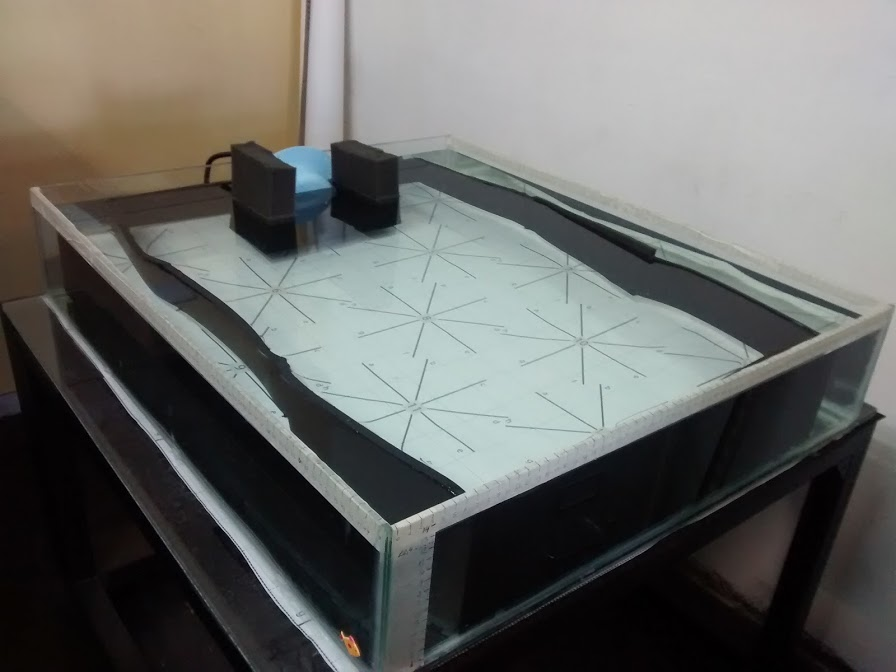
\includegraphics[height=6cm]{con_neoprene.jpg}
		\caption{Configuración con neoprene. La grilla observada debajo de la pecera corresponde a experimentos que no son de este proyecto y no afecta a ninguna de las mediciones realizadas.}
	\label{fig:conneo}
\end{figure}

Todas las caracterizaciones sin neoprene se realizaron durante Laboratorio 6 y el neoprene sólo se utilizó a partir de Laboratorio 7 . Sin embargo, durante el primer mes de Laboratorio 7 se repitieron las mediciones de la RI sin neoprene de las primeras cuatro filas de la grilla. Algún efecto que no se pudo identificar, probablemente sobreamplificación del parlante, no permitía separar la RI de la distorsión armónica.

\paragraph{Comentario sobre calibraciones:}
Todas las mediciones fueron realizadas utilizando una placa de sonido como dispositivo de adquisición. La placa de sonido mapea linealmente la tensión en la entrada de micrófono para que ocupe todo el rango de valores entre -1 y 1 con una resolución de 16 bits. Realizar una única calibración de tensión a valor mostrado en la PC es difícil ya que hay que considerar la ganancia del amplificador del hidrófono y el volumen de la PC, el cual además varía de una PC a otra. Para los estudios realizados esto no significa un problema ya que en todos los casos la variable de interés es la frecuencia medida y sólo interesan amplitudes relativas. Sin embargo, se determinó que para las configuraciones usadas (volumen máximo en PC y ganacia de 20x en el hidrófono), 30mV equivalen al máximo valor de amplitud en la escala de la PC. En lo que resta del informe, todas las amplitudes de sonidos medidas o generadas con la PC se mostrarán en unidades arbitrarias (del intervalo -1 a 1).

\section{Estudios comportamentales}
\subsection{Setup experimental, programa de adquisición y control}
Para los estudios comportamentales se delimitó una zona experimental en la primer mitad de la pecera utilizando el neoprene como se muestra en la figura \ref{fig:conneobis} (la elección se explica en la sección \ref{sec:rescompo} de los resultados y también se caracterizó la RI en esta configuración). El pez puede nadar libremente por la zona experimental y se lo estimula con algún sonido a intervalos de tiempo de 6 o 7 minutos. Un par de electrodos son conectados a un amplificador diferencial de ganancia 20x para medir la DOE y se filma al pez desde arriba con una cámara fotográfica a 40fps.

\begin{figure}[H]
	\centering
		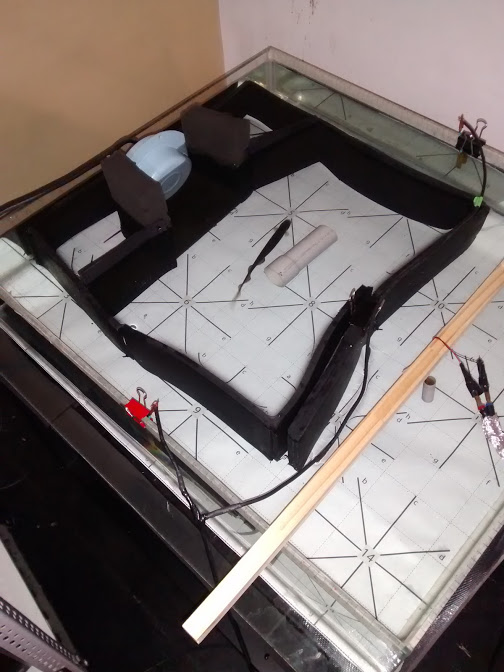
\includegraphics[width=6cm, height=6cm]{con_neo_bis.jpg}
		\caption{Configuración con neoprene utilizada para los estudios comportamentales. Sobre las paredes de la pecera se monta el par de electrodos y sobre la barra de madera el hidrófono y un LED (se enciende al emitir sonidos por el parlante y sirve como referencia visual del comienzo del estímulo en las filmaciones).}
	\label{fig:conneobis}
\end{figure}

La adquisición de datos y todo el control del experimento (salvo la filmación que es manual) se realiza a través de la placa de sonido de una PC mediante un programa escrito en Python 3.5. Utilizando la librería Sound Device y basándose en un ejemplo de su propia documentación [7] se adquiere la señal de la entrada estéreo de micrófono; son dos canales, uno utilizado para el par de electrodos y el otro para el hidrófono. Otro script que utiliza la librería PyAudio permite emitir tonos puros con frecuencia, duración y amplitud programados por el usuario y sonidos desde archivo (.wav). Una mínima interfaz de usuario muestra en un gráfico una ventana temporal de tamaño programable con las mediciones de los dos canales en tiempo real. El programa fué realizado en Laboratorio 7 y se planea su uso para otros experimentos realizados en el LFBM, tanto con peces eléctricos como dorados.

El único aspecto del setup que no fue automatizado es la filmación, ya que la cámara utilizada no cuenta con conexión a PC. Para sincronizar las filmaciones con los experimentos sin depender del volumen grabado por la cámara, se escribió un script para una placa Arduino que enciende un led cada vez que el programa de adquisición y control emite un estímulo. El led queda encendido durante toda la duración del estímulo, permitiendo ver en el video cuándo empieza y termina el sonido.

Todos los programas realizados se encuentran en el apéndice \ref{ap:programapython}.

\subsection{Condiciones de los experimentos}

Utilizando el mismo script de Matlab que genera las señales se prueba se hicieron diez barridos en frecuencia cortos para utilizar como estímulo. Todas las características de estos estímulos se encuentran listadas en la tabla \ref{tab:estimulos} (los barridos son llamados Sweeps). Se utilizaron también tonos puros de amplitud variable a 400Hz y 15ms de duración.

Los estímulos fueron aplicados en orden aleatorio y a intervalos de 6 a 7 minutos para prevenir la habituación del animal. El procedimiento para cada medición consiste en comenzar a grabar (único paso manual), adquirir la DOE durante algunos segundos y luego emitir el sonido con el programa de adquisición y control. La adquisición previa sirve de linea de base y sólo se requieren unos pocos segundos para determinar la frecuencia de descarga antes del estímulo (en ausencia de estimulación la frecuencia de descarga se mantiene constante). Todas las grabaciones se realizaron a 40fps ya que esta estapa de mediciones es exploratoria: sólo se busca saber con qué sonidos se puede gatillar la respuesta de escape o sobresalto y si hay correspondencia motora. En casos donde se requiere analizar la cinemática de la respuesta motora, las grabaciones se deben hacer a 240fps mínimo debido que a que la duración total de la respuesta es de 60ms a 80ms. Esto último no se realizó en este trabajo.

\begin{table}[H]
\centering
\resizebox{\textwidth}{!}{%
\begin{tabular}{c|c|c|c}
\doublerule
Tipo de estímulo        & Duración (ms)        & Frecuencia (Hz)                     & Amplitud (u. a.)         \\	\midrule
\multirow{10}{*}{Sweep} & 10                   & 500-1500                            & \multirow{10}{*}{1}      \\
                        & 15                   & 500-1500                            &                          \\
                        & 20                   & 500-1500                            &                          \\
                        & 25                   & 500-1500                            &                          \\
                        & 10                   & 500-1000                            &                          \\
                        & 15                   & 500-1000                            &                          \\
                        & 20                   & 500-1000                            &                          \\
                        & 25                   & 500-1000                            &                          \\
                        & 10                   & 500-8000                            &                          \\
                        & 15                   & 500-8000                            &                          \\	\midrule
\multirow{10}{*}{Tono}  & \multirow{10}{*}{15} & \multirow{10}{*}{400}               & \multicolumn{1}{c}{0.5}  \\
                        &                      &                                     & \multicolumn{1}{c}{0.55} \\
                        &                      &                                     & \multicolumn{1}{c}{0.6}  \\
                        &                      &                                     & \multicolumn{1}{c}{0.65} \\
                        &                      &                                     & \multicolumn{1}{c}{0.7}  \\
                        &                      &                                     & \multicolumn{1}{c}{0.75} \\
                        &                      &                                     & \multicolumn{1}{c}{0.8}  \\
                        &                      &                                     & \multicolumn{1}{c}{0.85} \\
                        &                      &                                     & \multicolumn{1}{c}{0.9}  \\
                        &                      &                                     & \multicolumn{1}{c}{0.95}	\\ \bottomrule
\end{tabular}%
}
\caption{Tabla de estímulos utilizados.}
\label{tab:estimulos}
\end{table}